\documentclass[a4paper,11pt,final]{article}
% Pour une impression recto verso, utilisez plutôt ce documentclass :
%\documentclass[a4paper,11pt,twoside,final]{article}

\usepackage[english,francais]{babel}
\usepackage[utf8]{inputenc}
\usepackage[T1]{fontenc}
\usepackage[pdftex]{graphicx}
\usepackage{setspace}
\usepackage{hyperref}
\usepackage[french]{varioref}
\usepackage{fancyhdr}
\usepackage{lastpage}
\usepackage{titlesec}
\usepackage[title,titletoc]{appendix}
\usepackage{rotating}

\newcommand{\reporttitle}{Rapport de projet Bataille Navale}     % Titre
\newcommand{\reportauthor}{Charles \textsc{Éponville}, Nicolas \textsc{Gille}, Vincent \textsc{Metton},$\newline$ Grégoire \textsc{Pommier}, Sylvestre \textsc{Vimard}} % Auteur
\newcommand{\reportsubject}{}  % Sujet
\newcommand{\HRule}{\rule{\linewidth}{0.5mm}}
\setlength{\parskip}{1ex} % Espace entre les paragraphes

\hypersetup{
    pdftitle={\reporttitle},%
    pdfauthor={\reportauthor},%
    colorlinks=false,
    pdfborder={0 0 0},
}

\titleclass{\subsubsubsection}{straight}[\subsection]

\newcounter{subsubsubsection}[subsubsection]

\renewcommand\thesubsubsubsection{\thesubsubsection.\arabic{subsubsubsection}}
\renewcommand\theparagraph{\thesubsubsubsection.\arabic{paragraph}}
\renewcommand\thesubparagraph{\theparagraph.\arabic{subparagraph}}

\titleformat{\subsubsubsection}
  {\normalfont\normalsize\bfseries}{\thesubsubsubsection}{1em}{}
\titlespacing*{\subsubsubsection}
{0pt}{3.25ex plus 1ex minus .2ex}{1.5ex plus .2ex}

\makeatletter
\renewcommand\paragraph{\@startsection{paragraph}{5}{\z@}%
  {3.25ex \@plus1ex \@minus.2ex}%
  {-1em}%
  {\normalfont\normalsize\bfseries}}
\renewcommand\subparagraph{\@startsection{subparagraph}{6}{\parindent}
  {3.25ex \@plus1ex \@minus .2ex}%
  {-1em}%
  {\normalfont\normalsize\bfseries}}
\def\toclevel@subsubsubsection{4}
\def\toclevel@paragraph{5}
\def\toclevel@paragraph{6}
\def\l@subsubsubsection{\@dottedtocline{4}{7em}{4em}}
\def\l@paragraph{\@dottedtocline{5}{10em}{5em}}
\def\l@subparagraph{\@dottedtocline{6}{14em}{6em}}
\@addtoreset{subsubsubsection}{section}
\@addtoreset{subsubsubsection}{subsection}
\@addtoreset{paragraph}{subsubsubsection}
\makeatother

\setcounter{secnumdepth}{5}
\setcounter{tocdepth}{5}

\begin{document}
  % Inspiré de http://en.wikibooks.org/wiki/LaTeX/Title_Creation

\begin{titlepage}

\begin{center}

\begin{minipage}[t]{0.48\textwidth}
  \begin{flushleft}
    
\includegraphics [width=75mm]{images/logo_univ.png} \\[0.5cm]
  \end{flushleft}
\end{minipage}

\textsc{\Large \reportsubject}\\[0.5cm]
\HRule \\[0.4cm]
{\huge \bfseries \reporttitle}\\[0.4cm]
\HRule \\[1.5cm]

\begin{minipage}[t]{0.3\textwidth}
  \begin{flushleft} \large
    \emph{Auteurs :}\\
    \reportauthor
  \end{flushleft}
\end{minipage}
\begin{minipage}[t]{0.6\textwidth}
  \begin{flushright} \large
    \emph{Responsable :} \\
    M.~Yannick \textsc{Guesnet} 
  \end{flushright}
\end{minipage}

\vfill

{\large \today}

\end{center}

\end{titlepage}

  \newpage
  \pagestyle{empty}
  \mbox{}
  \cleardoublepage % Dans le cas du recto verso, ajoute une page blanche si besoin
  \pagestyle{fancy}
  \fancyhf{}
  \fancyhead[LE,RO]{\reporttitle}
  \fancyhead[RE,LO]{L3 Informatique}
  \fancyfoot[CE,CO]{\reportauthor}
  \renewcommand{\headrulewidth}{2pt}
  \renewcommand{\footrulewidth}{1pt}
  \tableofcontents % Table des matières
  \newpage
  \listoffigures  % table des figures
  \sloppy          % Justification moins stricte : des mots ne dépasseront pas des paragraphes
  \cleardoublepage
  \setcounter{page}{1}
  \fancyfoot[LE,RO]{\thepage/\pageref{LastPage}}
  \section*{Remerciements}
\addcontentsline{toc}{section}{Remerciements}

Nous remercions : \newline
	M.GUESNET pour avoir proposé le sujet, nous avoir soutenu et encouragé tout au long du projet,\newline
	M.ANDARY pour avoir répondu à toutes nos question à propos de la manipulation des Threads en java,\newline
	M.BEDON pour avoir répondu à toutes nos questions quand au développement Java, serveur côté Java et l'utilisation des Threads,\newline
	M.VASSEUR pour avoir répondu à toutes nos questions liées à la partie réseau du projet.\newline
	Nous remercions aussi tout ceux qui nous ont aidés, apportés leur point de vue sur la tournure du projet, ou encore sur de potentielles idées d'améliorations.

  \cleardoublepage
  \section*{Introduction} % Pas de numérotation
\addcontentsline{toc}{section}{Introduction} % Ajout dans la table des matières
	De nos jours, il est possible de jouer à des jeux de société même avec des personnes qui ne sont pas dans la même pièce grâce aux différents protocoles réseaux. De plus en plus de jeux sont donc implémentés et utilisent ces technologies pour permettre de jouer en réseau, c'est à dire, de pouvoir jouer entre deux machines distantes. \newline

	De cette constatation, le besoin est venu d'implémenter un classique des jeux de société : la bataille navale (ou "touché coulé") qui est un jeu se jouant à deux joueurs dont le but est de couler tous les bateaux de l'adversaire, disposés sur un plateau de jeu. La bataille navale pouvant se jouer avec plusieurs règles, nous avons opté pour "le tour par tour" : chaque joueur joue une et une seule fois puis donne la main à son adversaire. \newline
	
	Ce projet a pour objectif de disposer de deux modes de jeu: un en local permettant de jouer contre une intelligence artificielle et l'autre permettant de jouer contre un adversaire humain en réseau.\newline
	
	Dans ce rapport, nous allons présenter les différents points de l'application, notamment en décrivant le modèle du jeu, ensuite la partie réseau, puis l'interface homme machine permettant à l'utilisateur de jouer dans des conditions correctes, enfin nous exposerons dans une dernière partie les différentes connaissances que ce projet a apporté, les difficultés rencontrées ainsi que l'évolution possible de ce projet.

  \cleardoublepage
  \section{Modèle de jeu}

\subsection{Le plateau de jeu}

	Dans le cadre de ce projet, nous avons choisi de donner aux joueurs la possibilité de jouer différemment à la bataille navale, notamment de jouer en trois dimensions.\newline
	
	Pour cela, nous avons réfléchi puis développé un modèle capable de s'adapter aux besoins des joueurs. En effet, celui-ci peut décider de toutes les tailles, longueur, largeur ou encore profondeur, ainsi qu'un nombre de dimensions quelconques. \newline
	
	Le plateau de jeu permet donc de jouer en une dimension (soit sur la longueur ou soit sur la largeur), en deux dimensions (longueur et largeur), en trois dimensions nous ajoutons la profondeur pour enfin pouvoir jouer en plus de trois dimensions.\newline
	
	\subsubsection{Définition récursive des Boards}
		Nous avons uns structure donnée qui se définit récursivement de la manière suivante : \newline
		\begin{itemize}
		\item Une case d'un Board est un Board à zéro dimensions.\newline
		\item Un Board à N dimensions, dont les tailles dans chaque dimension sont (TN, TN-1, … , T1) où les Ti sont les tailles, est composé de TN Boards à N - 1 dimensions, dont les tailles dans chaque dimension sont (TN-1, … , T1). 
		\end{itemize}
			
	Notez bien que les Boards à N - 1 dimensions ont exactement les même tailles pour chaque dimension. Ainsi, un Board à deux dimensions sera toujours représentable comme un rectangle, un Board à trois dimensions peut-être visualisé comme un pavé droit et ceux des dimensions supérieures suivent le même principe, bien qu'ils soient plus difficile à représenter.
\newline

	On peut aussi voir le Board comme un arbre particulier avec les propriétés suivantes : \newline
		\begin{itemize}
			\item La distance (plus court chemin de la racine à une feuille) et la hauteur (plus long chemin de la racine à une feuille) de l'arbre sont égales.\newline
			\item Tous les nœuds d'un même niveau ont le même nombre de descendants.
		\end{itemize}

	Cette structure récursive nous permet d'instancier un Board de n'importe quel nombre de dimensions en lui passant tout simplement un tableau d'entier classique contenant les tailles dans chaque dimension.

	\subsubsection{Remplissage des Boards}

	Pour remplir un tableau classique en programmation, on utilise généralement autant de boucles imbriquées qu'il y a de dimensions au tableau. Dans le cas du Board, ce n'est pas possible à notre connaissance, puisque le nombre de dimensions est inconnu à la compilation et qu'il faudrait un nombre variable de boucles imbriquées dans le code.\newline
	
	Nous avons donc créé un itérateur de Boards à nombre de dimensions zéro, implémenté dans la classe interne de Board, DimZeroIterator qui donne un par un les Boards à zéro dimensions qui sont les cases du Board. \newline

	Cet itérateur est également construit de manière récursive. Il contient les DimZeroIterator correspondants aux Boards fils du Board qu'il itère et les méthodes next() et hasNext() appelent leurs homologues sur l'itérateur fils en cours de parcours.

	Si on voit le Board comme un arbre, cet itérateur donne les cases dans l'ordre où un parcours en profondeur donnerait les feuilles.

	\subsubsection{Accès aux cases}

	L'accès en lecture et en écriture d'une case en particulier se fait grâce aux objets Coordinates.
Ces objets sont techniquement des tableaux d'entiers non mutables, dont on peut tester l'égalité avec la méthode equals() redéfinie. L'accès à une case de ce tableau se fait avec la méthode get(int index), à la façon des listes, mais il est itérable comme un tableau classique.\newline

	Lors d'un appel à getItem() ou setItem() sur un Board, chaque composante de la Coordinates fournie en paramètre sert à déterminer sur quel Board de dimension inférieure il faut effectuer l'appel récursif. \newline

	Les objets Coordinates sont également utilisés pour instancier les Boards en fournissant le nombre de dimensions et la taille pour chaque dimension.

	\subsubsection{Détails de l'implantation}

	Les algorithmes d'accès aux cases de Board sont récursifs terminaux; c'est à dire que lors de la compilation, le compilateur (si il y a compilation, ce qui est notre cas ici) peut remplacer ces appels récursifs par une simple boucle itérative. Cela s'explique par le fait que le rappelle a soi-même soit la dernière instruction a être évaluée. De ce fait, cela permet d'économiser de la mémoire lors des appels a ces fonctions, car seul l'adresse de l'appel de la fonction doit être sauvegarder sur la pile d'exécution. \newline
	Structures des objets :

	\begin{alltt}
	{\bf Structure} Board :
    	{\bf Champ} Object : item;
    	{\bf Champ} Liste de Board : boards;
	{\bf fin Structure}
		
	{\bf Structure} Coordinates :
    	{\bf Champ} Tableau d'entiers : coord;
	    {\bf Champ} Entier : length;
	{\bf fin Structure}
	\end{alltt}


	\subsubsubsection{Algorithmes de Coordinates}
	
	\begin{alltt}
{\bf Algo} Coordinates creerCoordinates(Tableau d'entier t) :
    coord <- copie de t;
	length <- longueur de t;
{\bf finAlgo}
			
{\bf Algo} Entier get(Coordinates c, Entier index) :
    renvoyer c.coord[index];
{\bf finAlgo}
	\end{alltt}

		
	\newpage
	\subsubsubsection{Algorithmes de Board}

	\begin{alltt}
{\bf Algo} Board creerBoard(Coordinates c) :
    renvoyer creerBoard(c, 0);
{\bf finAlgo}
		
{\bf Algo} Board creerBoard(Coordinates c, entier index) :
    Board b;
    b.item <- null;
    {\bf si} index = c.length {\bf alors}
        renvoyer b;
    {\bf finSi}
    b.boards <- nouvelle Liste de Board;
    {\bf pour} entier k de 0 à c.get(index) {\bf faire}
        b.boards[k] <- creerBoard(c, index + 1);
    {\bf finPour}
    renvoyer b;
{\bf finAlgo}
		
{\bf Algo} Object getItem(Board b, Coordinates c) :
    renvoyer getItem(b, c, 0);
{\bf finAlgo}
		
		
{\bf Algo} Object getItem(Board b, Coordinates c, Entier index) :
    {\bf si} index = c.length {\bf alors}
        renvoyer b.item;
    {\bf finSi}
    renvoyer getItem(b.boards.get(c.get(index)), c, index + 1);
{\bf finAlgo}
		
{\bf Algo} voidsetItem(Board b, Coordinates c, Object item) :
    setItem(b, c, 0, item);
{\bf finAlgo}
		
{\bf Algo} void setItem(Board b, Coordinates c, Entier index, Object item) :
    {\bf si} index = c.length {\bf alors}
        b.item <- item;
    {\bf finSi}
    setItem(b.boards.get(c.get(index)), c, index + 1, item);
{\bf finAlgo}
	\end{alltt}

\subsection{Les bateaux en dimensions variables}
	Les navires sont représentés par la classe Ship. Ils ont une longueur, un nom et contiennent les coordonnées des cases du Board qu'ils occupent lorsqu'ils sont placés. \newline

	Dans une bataille navale classique, chaque navire est disposé verticalement ou horizontalement. Dans notre modèle à nombre variable de dimensions, il faut généraliser cette règle pour qu'elle fonctionne dans tous les cas.

\subsubsection{Définition d'un bon placement}

	Pour être bien placés, les Ship doivent respecter les conditions suivantes :
	\begin{itemize}
		\item Bon alignement : les cases occupées par un Ship doivent avoir des coordonnées dont toutes les composantes sauf une sont égales, et les composantes qui ne le sont pas doivent se suivre. \newline
		Exemple : Dans un Board en quatre dimensions, un porte-avion (de longueur 5) occupe les cases (0,2,1,3), (0,2,2,3), (0,2,3,3), (0,2,4,3), (0,2,5,3). Ce placement respecte la condition de bon alignement car les premières, deuxièmes et quatrièmes composantes des coordonnés sont respectivement égales entre-elles, et que les troisièmes composantes se suivent. \newline
		
		\item Non dépassement : les cases occupées par un Ship sont celles contenues dans un Board. \newline
		Exemple : Dans un Board de dimensions (5,5,5,5), le porte-avion placé précédemment dépasse par sa dernière coordonnée, dont la troisième composante n'est pas comprise entre 0 et 4. \newline
		
		\item Bonne longueur : un Ship doit occuper exactement le même nombre de cases que sa longueur. \newline
		
		\item Non-Chevauchement : une case ne peut être occupée que par un seul Ship.
	\end{itemize}

\subsubsection{Tir sur les Ships}

	Les tirs sur les Ships se font via le Board sur lequel ils sont disposés. Pour cela, le type générique Board est paramétré soit par le type Case, soit par le type State. \newline
	
	Les Board<Case> de chaque joueur sont ceux sur lesquels ils placent leurs navires, et les Board<State> représentent la grille de tir des joueurs, là où ils peuvent voir où ils ont tirés et pour quel résultat. \newline
	
	State est une énumération représentant le statut de tir de chaque case d'un Board<State>. Il existe quatre états possibles :
	\begin{itemize}
		\item NOT$\_$AIMED : cette case n'a pas été visée par un tir.
		\item MISSED : il y a eu un tir sur cette case, mais il n'y avait pas de Ship adverse sur la case correspondante du Board<Case> du joueur adverse.
		\item HIT : Il y a eu un tir sur cette case, et un Ship adverse a été touché.
		\item SUNK : Même chose que HIT, avec en plus l'information que le Ship touché a été coulé par ce tir.
	\end{itemize}

	Les objets Case ont pour rôle de stocker deux informations : la présence d'un Ship et si la case a déjà reçu un tir. Ces deux informations suffisent à faire la distinction entre les états NOT$\_$AIMED, MISSED et HIT/SUNK. \newline
	
	Un objet Case sert également à relayer un tir jusqu'au Ship qui l'occupe, s'il y en a un, et à s'assurer qu'on ne tire pas deux fois au même endroit. Cette condition rend non-nécessaire le stockage dans les Ship des endroits précis où ils ont été touchés : un Ship qui a été touché un nombre de fois égal à sa longueur a forcément été touché sur toutes les cases qu'il occupe, et on sait ainsi qu'il a été coulé.\newline	
	
	Voici ce qui conclut la partie sur le modèles en tant que tels, vous avez vu comment est généré notre plateau de jeu ainsi, la façon dont on place nos bateaux sur cette grille de jeu ainsi que la façon dont se passe les tirs. Nous allons donc maintenant voir les intelligences artificielles développer dans le cadre du projet.
	
	\newpage

\subsection{Les intelligences artificielles}
	Il nous à été demandé de pouvoir jouer à la bataille navale en local. 
De ce fait, nous avons due développer une Intelligence Artificiel (IA), car jouer à deux sur un même ordinateur présente de nombreux risques de triches.\newline
	Notre IA se compose de 3 niveaux de difficultés différents, allant de facile à difficile.\newline
	Nous allons donc vous expliquez le fonctionnement de chacune de ces 3 IA.\newline

\subsubsection{IA Facile}
    L'IA facile fut la première intelligence artificielle programmée. Son cheminement est simple, elle consiste simplement à choisir aléatoirement une case, en vérifiant bien entendu que celle-ci n'est pas déjà était tirée au préalable, puis de tirer dessus, qu'importe l'avancement de la partie.\newline
    Le choix de l'aléatoire est fait de la façon suivante :\newline
    
\begin{alltt}
{\bf Fonction} EasyAdvisor :
	{\bf Entrée} : Board un tableau de state contenant les resultats de tous les tirs.
          Dim le tableau des tailles des dimension de Board.
    {\bf Sortie} : Coord une Coordonnée d’une case non touchée.
    {\bf Début}
        {\bf Faire}
            Entier distance = Alea(0, taille(Board)) ;
            Entier longueur = taille(Board) ;
            {\bf Pour} (n allant de 0 à taille(Dim))
                longueur = longueur / Dim[taille(dim) - 1 – n) ;
                Ajout(Coord, taille(dim) - 1 – n, distance / longueur) ;
                Distant = distance % longueur
            {\bf finPour}
        {\bf Tant que} (Board[Coord] != NON_CIBLÉ) ;
        Retourner Coord ;
    {\bf Fin}
{\bf Fin Procedure} 
\end{alltt}
        
\newpage        
        
\subsubsection{IA Moyen}
	L'IA moyen, deuxième IA développée, fonctionne de manière similaire à l'IA facile, à ceci près qu'une fois un bateau touché l'IA passe en mode "chasse".\newline
	Le mode chasse indique à l'IA de tirer sur les quatres directions(nord, sud, est et ouest) entourant la case touchée et, si une nouvelle case est touchée, celle-ci repart de cette dernière pour ainsi continuer jusqu'à avoir coulé le bateau.\newline
	Elle repart alors dans sa routine de ciblage.\newline
	L'algorithme est présenté ci-dessous:
    
\begin{alltt}
{\bf Procedure} MediumAdvisor :
    {\bf Entrée} : Board un tableau de state contenant les résultats de tous les tirs.
              Dim le tableau des tailles des dimension de Board.
              Coe une liste de case.
    {\bf Sortie} : Coord une Coordonnée d’une case non touchée.

    {\bf Début}
        {\bf Si} estVide(coe) 
            Coodinate c = EasyAdvisor(Board, Dim) ;
            {\bf SI} (Tir(enemy, c) != MANQUÉ)
                AjouterCasesAdjacentes(coe, coord) ;
            {\bf FinSi}
            Retourner Coord ;
        {\bf Sinon} 
            {\bf Si} (Board[Coe[0]] == NON_CIBLÉ)
                Coord = coe[0] ;
                Retirer(coe, 0) ;
                Retourner Coord ;
            {\bf FinSi}
            MediumAdvisor(Board, Dim, Coe);
        {\bf FinSi}
    {\bf Fin}
{\bf Fin Procedure}            
\end{alltt}

\newpage

\subsubsection{IA Difficile}
    L'IA difficile, troisième IA développée, fonctionne de manière similaire à l'IA normale, c'est à dire qu'elle effectue sa routine de "ciblage" jusqu'à toucher un bateau, puis passe en mode "chasse" une fois un bateau touché.
    La différence avec l'IA normale est que cette IA ne tire pas de case adjacente l'une à l'autre. En effet, suivant la taille minimal du bateau ennemi existant au début de partie, afin qu'elle ne tire que toute les tailles du bateau minimal.
    Par exemple, dans le cas ou le plus petit bateau est un bateau de 2, l'IA va donc écarter ses tirs de 2 cases d'écart à chaque fois.
    
\begin{alltt}
{\bf Procedure} HardAdvisor :
    {\bf Entrée} : Board un tableau de state contenant les résultats de tous les tirs.
              Dim le tableau des tailles des dimension de Board.
              Coe une liste de case.
              Minsize la taille du plus petit bateau présent sur la grille
    {\bf Sortie} : Coord une Coordonnée d’une case non touchée.

    {\bf Début}
        {\bf Si} estVide(coe)
            {\bf Faire}
                Entier distance = Alea(0, taille(Board)) ;
                Entier longueur = taille(Board) ;
                Entier mod = 0 ;
                {\bf Pour} (n allant de 0 à taille(Dim))
                    Mod = 0 ;	
                    longueur = longueur / Dim[taille(dim) - 1 – n) ;
                    Ajout(Coord, taille(dim) - 1 – n, distance / longueur) ;
                    Distant = distance % longueur
                    Mod = (mod + distance /longueur) % minsize;
                {\bf FinPour}
            {\bf Tant Que}(mod != 0 || Board[Coord] != NOTAIMED) ;

            {\bf SI} (Tir(enemy, coord) != MISSED)
                AjouterCasesAdjacentes(coe, coord) ;
            {\bf FinSi}   
            Retourner Coord ;
        {\bf Sinon}
            {\bf Si} (Board[Coe[0]] == NOTAIMED)
                Coord = coe[0] ;
                Retirer(coe, 0) ;
                Retourner Coord ;
            {\bf FinSi}
        {\bf FinSi}
        MediumAdvisor(Board, Dim, Coe) ;
    {\bf Fin}
{\bf Fin Procedure}
\end{alltt}
    
    Voici ce qui conclut notre première partie présentant le modèle de notre application, nous avons donc vu dans un premier temps le fonctionnement de notre grille de jeu, qui est donc une grille modulable à un nombre de dimension infini. Nous avons ensuite expliqué comment fonctionne nos bateaux, et la façon dont on tire dessus. Puis pour finir, nous avons montré le fonctionnement de nos IA ainsi que les différences entres les 3 niveaux de difficultés.
    Nous allons donc maintenant passer sur la seconde partie du projet qui est celle du réseau.
  \cleardoublepage
  \newpage
  \section{Le modèle réseau}

\subsection{Protocoles}
	\subsubsection{Protocole Réseau}
	Le protocole réseau\footnote{Tous les termes demandant explications sont disponibles dans le lexique} utilisé pour que deux joueurs puissent se connecter et jouer en réseau est le protocole TCP\footnote{Transmission Control Protocol : https://tools.ietf.org/html/rfc793} qui est un protocole en mode connecté mais également fiable quant à la connexion entre deux machines et pour la réception des paquets envoyés sur le réseau. \newline
	
	Nous avons préféré le protocole TCP au protocole UDP (\footnote{User Datagram Protocol : https://tools.ietf.org/html/rfc768} car, premièrement, son implémentation est bien plus aisée. En effet, nous n'avons pas à traiter certains cas d'erreurs, notamment dans le cas d'un paquet qui soit mal formé ou imcomplet car TCP assure que celui-ci sera totalement prêt avant de l'envoyer. \newline
	Deuxièmement, malgré le fait que le protocole UDP soit plus rapide dans l'envoi des données, utiliser le protocole TCP dans notre cadre n'a pas d'impact significatif puisque, comme il sera exposé un peu plus tard, chaque joueur doit attendre la réception de données avant de continuer son traitement. Ainsi, il n'est pas, en pratique, possible de recevoir des données qui ne sont pas attendues à des moments précis.

	\subsubsection{Protocole de l'application}
		L'application doit suivre un certain protocole pour que les deux joueurs puissent communiquer correctement et sans problèmes majeurs. Il a donc été décidé de suivre un type de protocole classique qui est celui du question/réponse. Néanmoins, nous n'avons pas choisi d'implémenter de serveur d'hébergement centralisant toutes les parties et dirigeant toutes les actions des clients, nous avons opté pour un échange de type pair à pair, c'est à dire que les deux joueurs doivent jouer les deux rôles: le processus serveur et le processus client, chacun à des temps déterminés et non mutables. \newline
		Nous expliquerons dans cette partie la connexion entre les deux joueurs ainsi que comment se passe l'échange de données.
		\subsubsubsection{Connexion des joueurs}
			Comme dit plus haut, chaque joueur doit jouer deux rôles bien distincts, celui du processus serveur comme celui du processus client. Dans ce cas-ci, il est donc bon de noter l'ordre des différentes opérations effectuées entre un joueur qui va accueillir la partie et celui qui va en être l'invité, nous allons donc expliciter quelles actions font parties du processus client et lesquelles font parties du processus serveur. \newline
			
			Les deux joueurs vont, en premier lieu, créer et lancer leur serveur respectif, en spécifiant l'adresse de la machine en format IPv4, un port d'écoute (nous vérifions qu'il soit compris entre 1024 et 65535), ainsi qu'un nombre de connexions autorisées qu'on nommera "backlog". \newline
			
			Ensuite, le joueur hôte met son serveur en attente d'une demande de connexion via sa socket d'écoute (il est donc considéré en tant que processus serveur) et, de son côté, le joueur invité (considéré comme le processus client à ce moment) va se connecter à l'adresse du joueur hôte. Cela aura pour effet, côté processus serveur, de créer une socket de service par laquelle le joueur passera pour communiquer avec le joueur invité. \newline
			
			À cette étape, il reste à faire la connexion inverse, c'est à dire que le joueur hôte (qui est maintenant le processus client) doit faire une demande de connexion à l'adresse du serveur du joueur invité (devenu le processus serveur) et, une fois la connexion acceptée par la socket d'écoute du processus serveur, une nouvelle socket de service est créée pour que le joueur invité puisse communiqué avec le joueur hôte.\newline
			
			Suite à ces différentes étapes, la connexion entre le joueur hôte et le joueur invité est établie, les échanges de données peuvent donc être effectuée.

		\subsubsubsection{Échanges des données}
			Mais avant de pouvoir commencer la partie et à échanger des données, chaque joueur doit placer ses bateaux puis attend que l'adversaire finisse de placer les siens. Pour nos besoins, nous n'avons pas décidé de laisser l'application choisir au hasard qui commence une partie: ce sera toujours le joueur hôte. \newline
			
			De ce fait, le joueur hôte devient donc le processus client qui doit alors choisir puis envoyer les coordonnées de son tir, ces dernières étant réceptionnées par le processus serveur, i.e le joueur invité, qui est en attente de ces coordonnées et rien d'autre. En effet, nous verrons plus tard comment ces données sont formatées pour que notre protocole fonctionne correctement (voir \ref{dataformat}).  \newline
			
			La prochaine étape consiste, pour le joueur invité maintenant devenu le processus client, d'envoyer le résultat du tir qui est un état de la case visée. Cet état peut être de trois natures: "touché", "coulé" ou bien "manqué". Le joueur hôte, quant à lui, attend l'arrivée de ce résultat en tant que processus serveur.\newline \label{states}
			
			Enfin, les joueurs mettent à jour leur vue respective pour finalement changer le tour de jeu, c'est à dire que le joueur hôte passe la main au joueur invité. \newline
			
			Ce schéma, se répète quand c'est au tour du joueur invité de jouer, il suffit simplement d'inverser les rôles pour obtenir un tour de jeu complet et ce jusqu'à la victoire d'un des joueurs qui fermeront correctement ensuite proprement les différentes sockets mises en jeu.
			
		\subsubsubsection{Format des données}
		\label{dataformat}
			Dans le cadre de notre protocole, il a fallu décidé d'un certain format que les données doivent respectées pour pouvoir être acceptées et ainsi traitées. De ce fait, tout paquet est formé de cette manière afin de faciliter l'extraction des données utiles au protocole:
			\begin{quote}
				"Objet:Valeur"
			\end{quote}
			Ces deux composantes définissent donc le format des données envoyées. Nous allons donc maintenant définir quels sont les types d'objets possible ainsi que leurs valeurs associées.
			
			\begin{enumerate}
				\item "Coordinates:X,X" $\Rightarrow$ Ce format permet d'envoyer les coordonnées d'un tir, la valeur est une suite de nombres séparés par des virgules représentant la coordonnée sur un axe donné. Par exemple, si nous recevons "Coordinates:1,1", cela signifie que nous voulons tirer sur la case situé à 1 sur l'axe des X et en 1 sur l'axe des Y.
			 
				\item "State:X" $\Rightarrow$ Ce format permet d'envoyer l'état de la case qui a été visé. Les valeurs possibles ont déjà été définies dans la partie \ref{states}. Par exemple, en recevant "State:HIT", cela signifie que la case visé à été touché.
				
				\item "String:X" $\Rightarrow$ Un objet String est une chaîne de caractères, la valeur pouvant être n'importe quelle chaîne. Grâce à ce format, nous pouvons envoyer des messages simples, comme le fait d'avoir gagné la partie ou bien un message d'erreur que nous affichons à l'utilisateur. 
				
			\end{enumerate}
			

\subsection{Gestion des erreurs}
	La gestion des erreurs est faites sur plusieurs niveaux d'abstraction dans notre projet. En effet, le premier niveau d'abstraction est le fait d'utiliser le protocole TCP/IP, car celui-ci, en opposition au protocole UDP, en plus de recevoir le paquet fait une vérification afin de valider le paquet avant de le transmettre. De ce fait, une partie des vérifications est déjà effectué par ce biais.\newline
	
	Le second niveau d'abstraction est lié au langage que nous avons choisi. En effet, Java implémente les protocoles TCP et UDP. Hors, Java effectue aussi des vérifications quand à la validité des données et permet facilement de vérifier si le paquet reçu est valide ou non, par le biais des Exceptions présente dans l'API de base.\newline
	
	Au final, nous avons implanté notre propre protocole de validité des données, afin d'être sur de ce que nous recevons. Comme vous avez pu le lire précédemment, chacune de nos données envoyées possède un format propre a notre protocole et si, lors d'un envoie de donnée, nous n'avons pas le bon type de données, alors nous gérons le problème en indiquant qu'un problème est survenue lors de l'envoie des données, ce qui n'est pas normal et qui indique un problème au niveau du programme. De ce fait, nous fermons donc proprement l'application afin d'éviter tout problèmes lors d'une exécution prolongée du logiciel.

  \cleardoublepage
  \section{Interface Homme Machine}
	Dans toute application où les interactions avec l'utilisateur sont fréquentes, et notamment dans un jeu tel que la bataille navale, il est bon que cette application possède une interface homme machine(IHM) qui va prendre en compte les actions de l'utilisateur et modifier ce qu'il voit en conséquence. \newline
	
	Nous avons donc développé une IHM permettant à un joueur de pouvoir jouer aisément et sans difficultés qui va se découper en deux fenêtres principales. La première est la fenêtre de démarrage où l'utilisateur pourra définir les différentes options liées à la nouvelle partie et la seconde est l'interface principale du jeu où toute la partie se déroulera. Nous allons donc exposer ces deux fenêtres dans deux parties distinctes où nous expliquerons comment les fenêtres sont construites et détaillerons les différents actions a effectué. Enfin, nous en profiterons pour mettre en avant, dans une troisième partie, les composants graphiques permettant l'affichage des Boards. 
	
\subsection{La fenêtre de démarrage}
	Comme dit plus haut, la fenêtre de démarrage est la première fenêtre que verra le joueur au lancement de l'application. Pour nous aider à décrire cette fenêtre, voici une capture d'écran:
	
	\begin{figure}[!h]
		\centering
		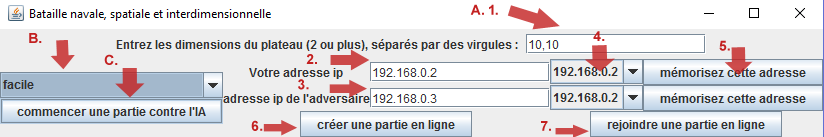
\includegraphics [width=10cm]{images/start_window.png}
		\caption{Fenêtre de démarrage de l'application}
		\label {startwindow}
	\end{figure}
	
	Comme on peut le voir, la fenêtre de démarrage est séparée en plusieurs morceaux. Pour s'y repérer, nous allons d'abord nous intéresser aux différents champs à remplir et actions à effectuer pour pouvoir créer une partie locale contre une IA, puis nous réitérerons cette logique pour pour soit créer, soit rejoindre une partie en ligne.
	
	\subsubsubsection{Une partie en local}
		Pour effectuer une partie en local, il faut premièrement indiquer, dans le champ de texte en haut à droite symbolisé par un "A", les dimensions de notre plateau de jeu, chaque dimension étant séparée par le symbole ",". Puis, nous devons choisir, grâce à la liste déroulante symbolisé par un "B" à gauche, le niveau de difficulté choisi pour l'IA qui sont, à l'heure actuelle, au nombres de trois. Enfin, Nous pouvons lancer la partie en cliquant sur le bouton "commencer une partie contre l'IA, qui se situe en bas à gauche symbolisé par un "C".

	\subsubsubsection{Une partie en réseau}
		Pour pouvoir jouer ligne, il faut, bien entendu, indiquer les dimensions du plateau de jeu, cependant cette information n'est nécessaire que pour le joueur qui hébergera la partie. Comme pour la partie en local, il faut remplir le champ de texte marqué d'un "1" en haut à droite de la fenêtre. Ensuite, chaque joueur doit rentrer son adresse IPv4 dans le champ numéroté "2" et l'adresse IPv4 de l'adversaire dans le champ numéro "3" au centre de la fenêtre. \newline
Il est également possible de récupérer une adresse mémorisé au préalable dans un fichier texte, apparaissant dans les liste déroulantes notés "4" mais aussi de mémoriser l'adresse, qui est écrite dans les champ de textes sus-mentionné, grâce aux boutons sur la droite.
\newline
Enfin, le joueur hôte lance la partie en cliquant sue le bouton "créer une partie en ligne", noté "6" en bas au centre de la fenêtre et le joueur invité peut rejoindre une partie après avoir cliqué sur le bouton indiqué par un "7".

\subsection{L'interface du jeu}
	\subsubsection{Le placement des bateaux}
		Avant de pouvoir jouer, il est nécessaire que les joueurs puissent placer leurs bateaux. Ce placement est illustré dans la figure suivante: \newline
		\begin{figure}[!h]
			\centering
			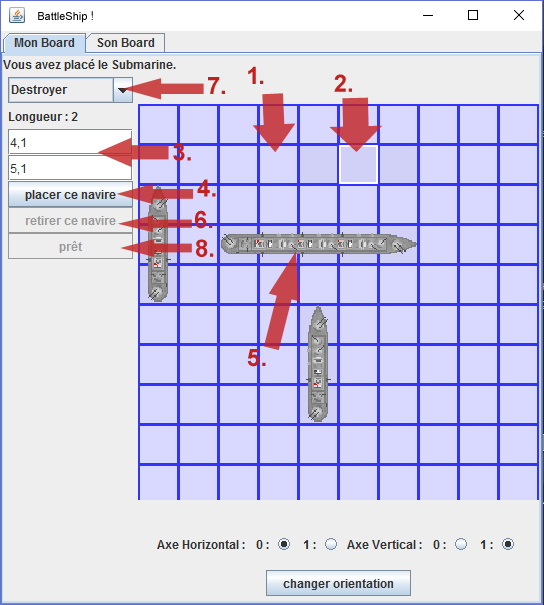
\includegraphics [width=5cm]{images/ship_placement.png}
			\caption{Placement des bateaux}
		\end{figure}
	
	Le  joueur doit avant tout cliquer sur une des cases du plateau de jeu, ce composant graphique un peu spécial sera explicité dans une autre sous-partie. La case cliquée représentera alors la proue du bateau("1") et, en cliquant sur une seconde case, nous choisissons la poupe("2") de celui-ci. Il est à noter que, sur la gauche de la fenêtre, il est possible d'entrer les coordonnées des deux cases en format textuelle, c'est à dire "X,X"("3").
	\newline
	
	Il faut ensuite cliquer sur le bouton "Placer ce navire"("4"), en dessous des champs de texte permettant de renseigner les coordonnées. Le fait de cliquer sur ce bouton a pour effet de faire passer le bateau a placé au suivant dans la liste déroulante en haut à gauche("7"). Naturellement, il est aussi possible de retirer un navire précédemment placé en le choisissant dans cette même liste et en cliquant dur le bouton "retirer ce navire" ("6").
	\newline
	
	Enfin, une fois tous les bateaux placés, le bouton "prêt"("8") est activé et nous pouvons cliquer dessus pour débuter une partie.
	\newline
	
	Toutes ces étapes même au commencement de la partie. Nous allons donc maintenant décrire ce que l'utilisateur voit et peut faire lors d'un tour de jeu sur une partie déjà avancée.
	
	\subsubsection{Une partie typique}
	Pour comprendre l'interface mise en œuvre ici, il est nécessaire de pouvoir la visualiser correctement. Pour cela, une capture de la fenêtre est donnée ci-après:\newline
	\begin{figure}[!ht]
		\centering
		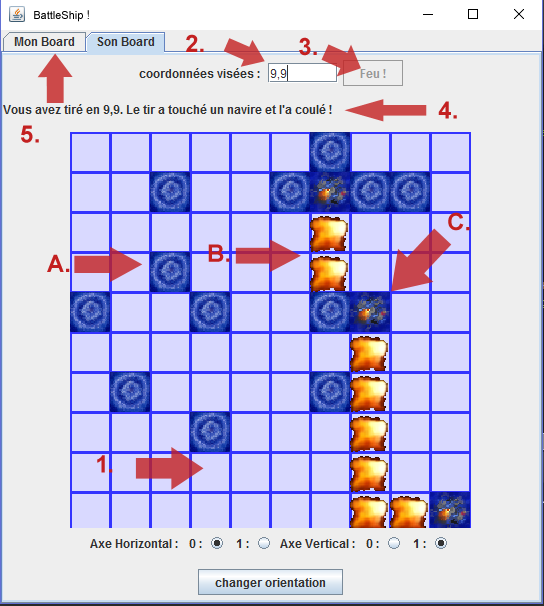
\includegraphics [width=5cm]{images/game_in_action.png}
		\caption{Une partie à un stade avancée}
	\end{figure}
	
	Sur cette image, nous pouvons tout d'abord parler du plateau de jeu. En effet, celui ci voit ses cases changées au cours de la partie suivant si la case a été ciblé on non ("1"). Si elle a été ciblé, cette case peut marqué comme "manqué" ("A"), "touchée" ("B") ou ecnore "coulée" ("C").
	\newline
	
	Lors du tour du joueur, celui-ci doit renseigner la case ou les coordonnées sur lesquelles il souhaite tirer. Il a donc à sa disposition la possibilité de soit cliquer directement sur la case voulue("1") ou alors de rentrer les coordonnées de la case au format textuel comme défini plus haut ("2"). Le joueur fait ensuite feu grâce au bouton "Feu!" ("3") et obtient le résultat de son tir qui affiche donc une image différente pour les trois cas possibles("A", "B" ou "C") ainsi qu'un petit texte décrivant la nature du résultat ("4"). Le joueur a également la possibilité de regarder son plateau de jeu, en cliquant sur l'onglet "Mon Board" ("5").
\newline

	Voici typiquement comment l'IHM s'arrange et les différentes actions que le joueur peut effectuer au cous d'une partie. 
	 \newline
	  
	Nous allons maintenant évoqué et expliqué le composant graphique majeur de l'application, le plateau de jeu qui se décline en plusieurs composants suivant quel plateau nous souhaitons regarder: soit le notre avec la position de nos bateaux, soit celui de l'adversaire contenant tous les résultats de nos tirs.

\subsection{La représentation du plateau de jeu}
	La représentation d'un espace à deux, trois ou plus de dimensions se complexifie avec le nombre de dimensions.
Nous avons choisi de représenter les plateaux à deux dimensions de manière classique, une surface avec un quadrillage. La représentation des plateaux à trois dimensions utilise une succession de plateaux à deux dimensions empilés entre lesquels on peut naviguer facilement. \newline

	Pour les nombres de dimensions supérieures, nous avons fait le choix de ne pas tout représenter étant donné la difficulté de visualiser un espace à quatre dimensions pour les humains et l'absence de conventions communément partagées sur la représentation de cet espace.

\subsubsection{Explications sur les axes}

	Plutôt que de montrer une représentation qui ne serait pas comprise par les joueurs, nous avons opté pour un système de composantes fixes pour les dimensions non représentées. Ainsi, pour représenter un Board de dimensions (5, 5, 5, 5), on peut fixer la quatrième composante de chaque case représentée à la valeur t : les cases représentées seront celles dont les coordonnées sont (x, y, z, t) pour x, y et z entre 0 et 4, et pour t fixé. Les cases de coordonnées dont la quatrième composante n'est pas égale à t ne sont pas représentées.
\newline

	Nos composants graphiques utilisent des objets Coordinates d'une façon spéciale pour déterminer les axes et les coordonnées fixées.
	\newline	
	
	Dans ces coordonnées, les composantes de valeurs positives ou nulles représentent des composantes fixées et les valeurs -1, -2, -3 désignent respectivement qu'il faut représenter les composantes correspondantes sur l'axe X (horizontal, de gauche à droite), l'axe Y (vertical, de haut en bas) ou sur l'axe Z (en profondeur, vers l'écran).
\newline
	
	Exemple : Dans une représentation en 3 dimensions d'un Board de dimensions (5, 4, 5, 3, 6), si on fixe l'axe à (-1, 2, -3, 1, -2). Les cases représentées seront celles de coordonnées (a, 2, b, 1, c) avec a, b et c des valeurs entières dans les limites des dimensions du Board.
Chaque case sera représenté sera située à la a-ième place sur l'axe des X, la c-ième place sur l'axe des Y et la b-ième place sur l'axe des Z.
\newline

	Dans la suite et dans le code source, nous appelons "axes" ces objets qui déterminent quelles composantes sont représentées sur quels axes et lesquelles sont fixées.

\subsubsection{Représentation en deux dimensions : les GraphicBoards}


	Un objet GraphicBoard est un JComponent permettant la représentation en deux dimensions, il connaît le Board qu'il représente ainsi qu'un axe pour déterminer quelles cases du Board il doit représenter et dans quel sens. \newline

	En plus de ça, le GraphicBoard contient deux modes d'interaction : un passif et un actif.
Le mode passif répond aux clics de souris en envoyant un événement simple dont la sémantique est tout simplement "on m'a cliqué dessus". \newline

	Le mode actif répond aux clics de souris par un CoordinatesEvent contenant les coordonnées de la case cliquée dans le modèle du Board. Ce ne sont pas les coordonnées "graphiques" mais bien celles correspondantes à la case du Board dont on a cliqué sur la représentation graphique.

\subsubsection{Représentation en trois dimensions : Les GraphicBoardLayers}
	Un GraphicBoardLayer est un JPanel contenant plusieurs GraphicBoards en couches superposées.
Il permet de naviguer entre ses couches de plusieurs manières : en cliquant sur la couche qu'on veut voir entièrement (elles sont toujours cliquables car la superposition est en décalé), en utilisant le slider sur le coté ou avec la molette de souris.
\newline

	Le GraphicBoardLayer s'assure qu'un seul GraphicBoard est en mode d'interaction actif et qu'il soit entièrement visible (en décalant ceux du dessus).
	\newline
	
	Il contient également des options de changement de la représentation, comme les changements d'axes, avec des boutons radios, et dans le cas où le Board qu'il représente contient plus de trois dimensions, il permet de fixer les composantes non représentées sur les axes.
\newline

Le GraphicBoardLayer relaie les CoordinatesEvents du GraphicBoard en mode actif.

\subsubsection{Délégation de l'affichage spécifique : les BoardDrawer}

	GraphicBoard et GraphicBoardLayer sont des classes génériques, aptes à représenter les plateaux sur lesquels sont placés les navires comme les plateaux de tir. L'affichage spécifique de chaque type de plateau ne peut donc pas être prise en charge.\newline
	
	Cet affichage est donc délégué à des objets de type BoardDrawer, qui est une interface elle aussi générique, mais que nous avons implanté en deux classes non génériques, ShipDrawer et ShootDrawer.

\subsubsection{La représentation des tirs : GraphicBoardShooter}

	Le GraphicBoardShooter contient un GraphicBoardLayer dont il récupère les CoordinatesEvents pour remplir un champ de coordonnée de tir.
Il est doté d'un bouton "feu" qui s'active si les deux conditions suivantes sont remplies :
\begin{itemize}
\item La case correspondante aux coordonnées actuelles n'a pas encore été visée.
\item C'est le tour du joueur (attribut booléen myTurn qui passe systématiquement à Faux après un tir, et que le contrôleur de jeu peut passer à VRAI ou FAUX) : C'est ce contrôleur (LocalController ou SuperController) qui donne donc l'autorisation de tirer avant chaque tir.
\end{itemize}


Comme tout n'est pas forcément visible, un label indique la dernière coordonnée de tir et son effet sur l'adversaire (s'il a touché ou coulé un navire).

\subsubsection{La représentation des navires : GraphicShipBoard}

	Le GraphicShipBoard contient lui aussi un GraphicBoardLayer dont il récupère les CoordinatesEvents pour remplir tour à tour deux champs de coordonnées (c'est-à-dire qu'il remplit le premier au premier événement, le second au second événement, puis de nouveau le premier, etc). \newline
	
	Avec ces deux champs de coordonnées qui représentent les coordonnées potentielles des extrémités d'un navire, le joueur peut essayer de placer le navire actuellement sélectionné dans la liste déroulante, s'il n'est pas déjà placé.
Si les conditions d'un bon placement de navires sont réunies, le navire sera alors placé, sinon, un message s'affichera, expliquant pour quelle raison le navire n'a pas pu être placé.
\newline
	Lorsque tous les navires sont placés et que le joueur clique sur le bouton "prêt", le panneau de placement des navires disparaît.
	Le GraphicShipBoard représente les tirs subis en plus des navires. \newline
	
	Nous avons donc vu ensemble la partie graphique de l'application, de son démarrage jusqu'au déroulement d'une partie classique. Il nous reste une dernière partie à présenter, qui est la partie "humaine" du projet, c'est à dire les choses que nous avons acquit au cours du projet, les divers problèmes rencontrées, les idées d'améliorations potentielles ainsi que les technologies que nous avons utilisées tout au long du projet.
  \cleardoublepage
  \section{Autres}

\subsection{Technologies utilisés}
	Les technologies que nous avons utilisé durant le projet sont les suivantes.\newline
	La première technologie utilisée fut le langage Java. En effet, nous avons choisit de prendre le Java, car notre client nous l'a conseillé, en particulier pour ce qui est la gestion de l'IHM. De plus, étant un langage que nous maîtrisons tous plus ou moins, nous avions ainsi davantage de facilité à le manier et donc à développer le projet voulu.\newline
	La seconde technologie fut l'utilisation de GIT, un logiciel de gestion de version de code source. En effet, via GIT, nous pouvions aisément travailler sur des partie du code différentes sans interférer avec les autres. De plus, cela nous permettait, en cas de soucis, de récupérer le code ultérieur pour repartir dessus si des améliorations, ou des modifications apportées au code courant modifièrent trop le fonctionnement de l'application, ou pire, créèrent des bugs non réparable.\newline
	La troisième technologie que certains d'entre nous apprirent fut \LaTeX{}, car part le biais de \LaTeX{}, nous avons pu rendre un rapport de projet propre, et surtout facilement modifiable en cas de besoin.

\subsection{Idées d'améliorations}
	Voici une liste d'amélioration possible qui pourrait être implanter sur le projet afin de le rendre encore plus complet.\newline
	La première amélioration serait d'ajouter une IA très difficile, qui fonctionnerait de la même façon que l'IA difficile, avec cependant une variante qui consisterait à adapter les coups qu'elle tire en fonction des bateaux touchées et des cases restantes sur la grille.\newline
	La seconde amélioration possible serait le fait qu'un thread utilisateur soit lancer lorsque nos sockets de service sont en attendent. En effet, lorsque celles-ci sont en attente, EDT (Event Dispatch Thread) le thread gérant toute l'IHM se retrouve aussi bloquer due a l'attente de réception de données.\newline
	Une troisième amélioration potentielle serait d'améliorer l'IHM afin que celle-ci affiche un beau menu lors de l'ouverture du logiciel, afin que les utilisateurs ait vraiment la sensation de jouer à un jeu.\newline
	Nous pourrions aussi ajouter le Drag'n'Drop, appelé aussi "Glissé-Déposé", pour placer plus facilement nos bateaux sur la grille, lors du début d'une partie. En effet, nous plaçons actuellement nos bateaux par le biais d'un clique plaçant l'avant du bateau, puis l'arrière du bateau par un second clique, et le fait de le faire par Drag'n'Drop serais plus intuitifs pour certaines personnes.\newline
	Il serait aussi possible d'offrir la liberté d'ajouter plus de bateaux, ou de modifier ceux existant, par exemple en modifiant leur taille, ou encore en jouant avec 7 bateaux au lieu de 5 initialement dans les règles officiels de la bataille navale.\newline
	Une autre amélioration développable serait de pouvoir changer les règles ou d'ajouter des règles durant une partie. Par exemple, nous pourrions utiliser ajouter un chronomètre lors d'un tour de jeu, afin que chaque joueur doivent jouer rapidement, sous peine de voir son tour être passé sans avoir eu le temps de jouer.
	Nous pourrions aussi ajouter un chat pour que les joueurs puissent communiquer entre eux, afin qu'ils puissent par exemple discuter entre eux, ou encore se charrier gentillement lors d'un coulé par exemple.\newline
	Comme nous l'avons vu, ce projet ne possède guère de limite si ce n'est notre imagination.\newline

\subsection{Problèmes rencontrés}
	De nombreux problèmes ont été rencontrés au cours du projet, les plus important d'entre eux sont le fait que nous avons manquée de temps pour le projet, ainsi que le manque de salle informatique pour travailler efficacement, notamment le vendredi après midi, ou aucune salle informatique n'était libre pour nous permettre de bosser tous ensemble.\newline
	Un autre problème que nous avons rencontré est le fait que nous n'avions pas de redirection de port, ne permettant pas de tester facilement la partie réseau du projet, car il faut absolument que chacun possède son point d'accès, pour pouvoir le modifier, ce qui n'était pas forcément le cas.\newline
	Nous avons rencontré aussi des problèmes organisationnelles et logistiques vis à vis du travail de chacun au début, en particulier sur le début du projet.\newline
	Au niveau du développement, nous avons rencontré un problème au niveau de l'uniformisation du code. En effet, nous avions convenu initialement de coder en anglais, langue universelle de l'informatique. Hors, plusieurs fois nous nous somme rencontrer a des noms de variables ou encore de méthodes écrite en français, faisant ainsi une grosse différence entre chaque développeur présent sur le projet.\newline
	Toujours au niveau du code, nous avons eu de grosse difficultés à manipuler les threads, en particulier le lien entre EDT et les thread utilisateurs, ce qui explique que cette gestion n'ait pas été réalisé et implanter dans le code, malgré de nombreuses heures passées dessus.\newline
	Pour terminer, une dernière difficulté s'est aussi présenté à nous, en effet, l'appréhension et la visualisation du modèle permettant des grilles à dimension variable et inconnu a été assez difficile a comprendre, car au delà de la troisième dimension, nous étions régulièrement perdu.

\subsection{Compétences acquises}
	Au cours du projet, nous avons acquit nombres de connaissances tels que par exemple l'initiation a GIT, un logiciel de versionning de code, permettant ainsi un travail efficace en groupe, car chacun peut facilement travailler sur un module du projet sans risquer de "casser" le code fonctionnel.\newline
	 Nous avons aussi acquit de nombreuses connaissances sur le réseau, en particulier sur le protocole TCP/IP qui est un standard d'internet, ainsi que le fonctionnement d'un protocole question/réponse et pour finir l'utilisation des sockets par le biais du langage Java.\newline
	 Pour finir, nous avons acquit la capacité de gérer et de se répartir le travail efficacement lorsqu'on travail en groupe.
  \cleardoublepage
  \section*{Conclusion}
\addcontentsline{toc}{section}{Conclusion}

	Ce projet s'est révélé très enrichissant dans la mesure ou nous avons pu utilisés toutes nos compétences afin de produire une application la plus fonctionnelle, la plus propre et la plus adapté au besoin de notre client M.GUESNET.\newline
	Ce projet nous a aussi permis de mettre en corrélation la partie théorique et pratique vu en cours afin de produire un projet complet, reliant divers aspect de l'informatique, nous pensons notamment à la partie réseau, couplée a l'IHM et au modèle MVC que nous avons étudiez jusqu'ici.
	Nous avons acquis nombre de nouvelles compétences qui nous seront très utile dans nos projets futurs, nous pensons notamment à GIT, qui est un outil extrêmement puissant et efficace quand il s'agit de travailler en groupe, ou encore a \LaTeX{}, qui nous permettra de rendre des rapports très beau et fonctionnel.\newline
	Tout en restant positif, nous n'oublions pas les nombreuses difficultés que nous avons rencontrées tout au long du projet, à savoir principalement la difficultés de travailler dans un groupe, être capable d'uniformiser le code, ou l'apprentissage de nouvelles technologies.\newline
	Pour conclure, nous souhaitons que notre production soit appréciées par tous et qu'un jour, des développeurs aient envie de reprendre le projet afin de l'améliorer.
	

  \cleardoublepage
  \newpage
\begin{appendices}
\section{Lexique}
\begin{itemize}
	\item EDT~:
	EDT est un acronyme signifiant Event Dispatch Thread. Concrètement, EDT est le thread principal s'occupant de la partie graphique d'une application Java, c'est-à-dire le dessin de l'IHM ou la gestion des interactions avec l'utilisateur.
	\newline

	\item Itérateur~:
	En programmation, un itérateur est un objet permettant de parcourir un tableau ou une collection, non pas nécessairement depuis le début du tableau, mais depuis n'importe quel index du tableau. Dans le cadre de notre projet, notre itérateur nous permet de parcourir notre Board.
	\newline

	\item Pair à pair~:
    Le pair à  pair (ou peer-to-peer en anglais), est un modèle de réseau permettant à deux machines de discuter d'égale à égale.
    Dans les faits, cela s'explique par le fait qu'une machine se connecte à une autre machine et inversement afin que celles-ci puissent s'échanger des informations sans passer par un serveur distant.
    \newline
    
   	\item Protocole réseau~:
    Un protocole est une méthode standard qui permet la communication entre des processus (s'exécutant éventuellement sur différentes machines), c'est-à-dire un ensemble de règles et de procédures à respecter pour émettre et recevoir des données sur un réseau. 
    Il en existe plusieurs selon ce que l'on attend de la communication. Certains protocoles seront par exemple spécialisés dans l'échange de fichiers (le FTP), d'autres pourront servir à gérer simplement l'état de la transmission et des erreurs (c'est le cas du protocole ICMP), ... 
	\newline

	\item Protocole TCP~: 
    Acronyme de Transmission Control Protocol, le protocole TCP/IP est le protocole standard utilisé sur internet, pour la liaison entre deux ordinateurs.
    Le protocole TCP vérifie la validité des paquets après leur réception afin d'être sûr de la validité de celle-ci.
    Le protocole TCP est située sur la couche 4 (couche de transport) du modèle OSI. 
	\newline
	
	\item Protocole UDP~:
    Acronyme User Datagram Protocol, le protocole UDP est un des protocoles standards utilisé sur internet. 
    La différence avec TCP est que les paquets sont reçus sous forme de datagrammes qui doivent être vérifiés pour valider la qualité du paquet reçu.
    Le protocole UDP est très utilisé, notamment, dans le cadre du jeu en ligne, ou encore le streaming, car la perte de paquet influe peu sur la quantité reçus.
    Le protocole UDP est située sur la couche 4 (couche de transport) du modèle OSI, au même titre que le protocole TCP. 
   \newline

	\item Socket~:
    Une socket est une interface de connexion bidirectionnelle permettant l'échange de données entre deux processus (distants ou non).
	\newline
 
	\item Socket de Berkeley~:
    Les sockets de Berkeley, sont un ensemble normalisés de fonctions de communications lancé par l'université de Berkeley au début des années 1980.
    De nos jours, elle est la norme utilisé par quasiment l'ensemble des langages de développement (C, Java, Python, ...).
    \newline
  
	\item Socket d'écoute~:
    Une socket d'écoute est une socket présente uniquement dans le protocole TCP. En effet, son rôle consiste, comme son nom l'indique, à écouter les demandes de connexion de socket externe sur un port prédéfini, afin de créer une socket qui permettra ensuite l'échange de données avant de reprendre son rôle d'écouteur.
	\newline
  
	\item Socket de service~:
    La socket de service est la socket crée par la socket d'écoute lorsque celle-ci reçoit une demande de connexion. La socket de service permet la communication entre le serveur et le client ayant fait une demande de connexion. C'est par cette socket que transitent toutes les données émises par le client et le serveur.
	\newline
  
	\item Thread~:
	Un thread est une sorte de processus, dit "léger". Le rôle d'un thread est d'exécuter une suite d'instruction précise que l'on peut nomme routine.
	Le fait de lancer une application informatique lance automatiquement un thread, celui-ci peut alors créer d'autres threads afin de délégué par exemple une tâche longue a un autre thread, afin que le thread principal (main thread), puisse continuer son fil d'exécution à lui.
	\newline

   
\end{itemize}


\newpage
\section{Webographie}
\begin{itemize}
	\item Fonctionnement des intelligences artificielles~: \url{http://www.datagenetics.com/blog/december32011/index.html}
\newline	
	\item API Java~: \url{https://docs.oracle.com/javase/7/docs/api/}
	\newline
	\item Règles de la bataille navale: \url{http://www.regles-de-jeux.com/regle-de-la-bataille-navale/}
\end{itemize}

\newpage
\section{Schéma du protocole de l'application}
\begin{sidewaysfigure}
    \centering
    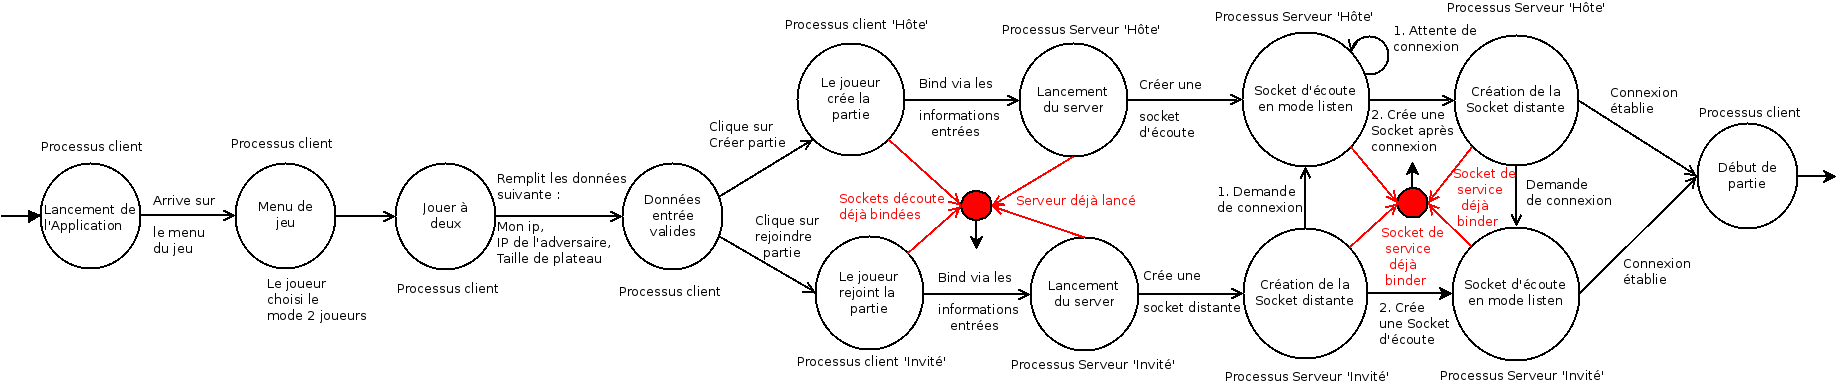
\includegraphics [width=215mm]{images/connection_between_players.png}
    \caption{Schéma représentant le protocole de connexion entre deux joueurs}
    \label{connection}
\end{sidewaysfigure}
\begin{sidewaysfigure}
    \centering
    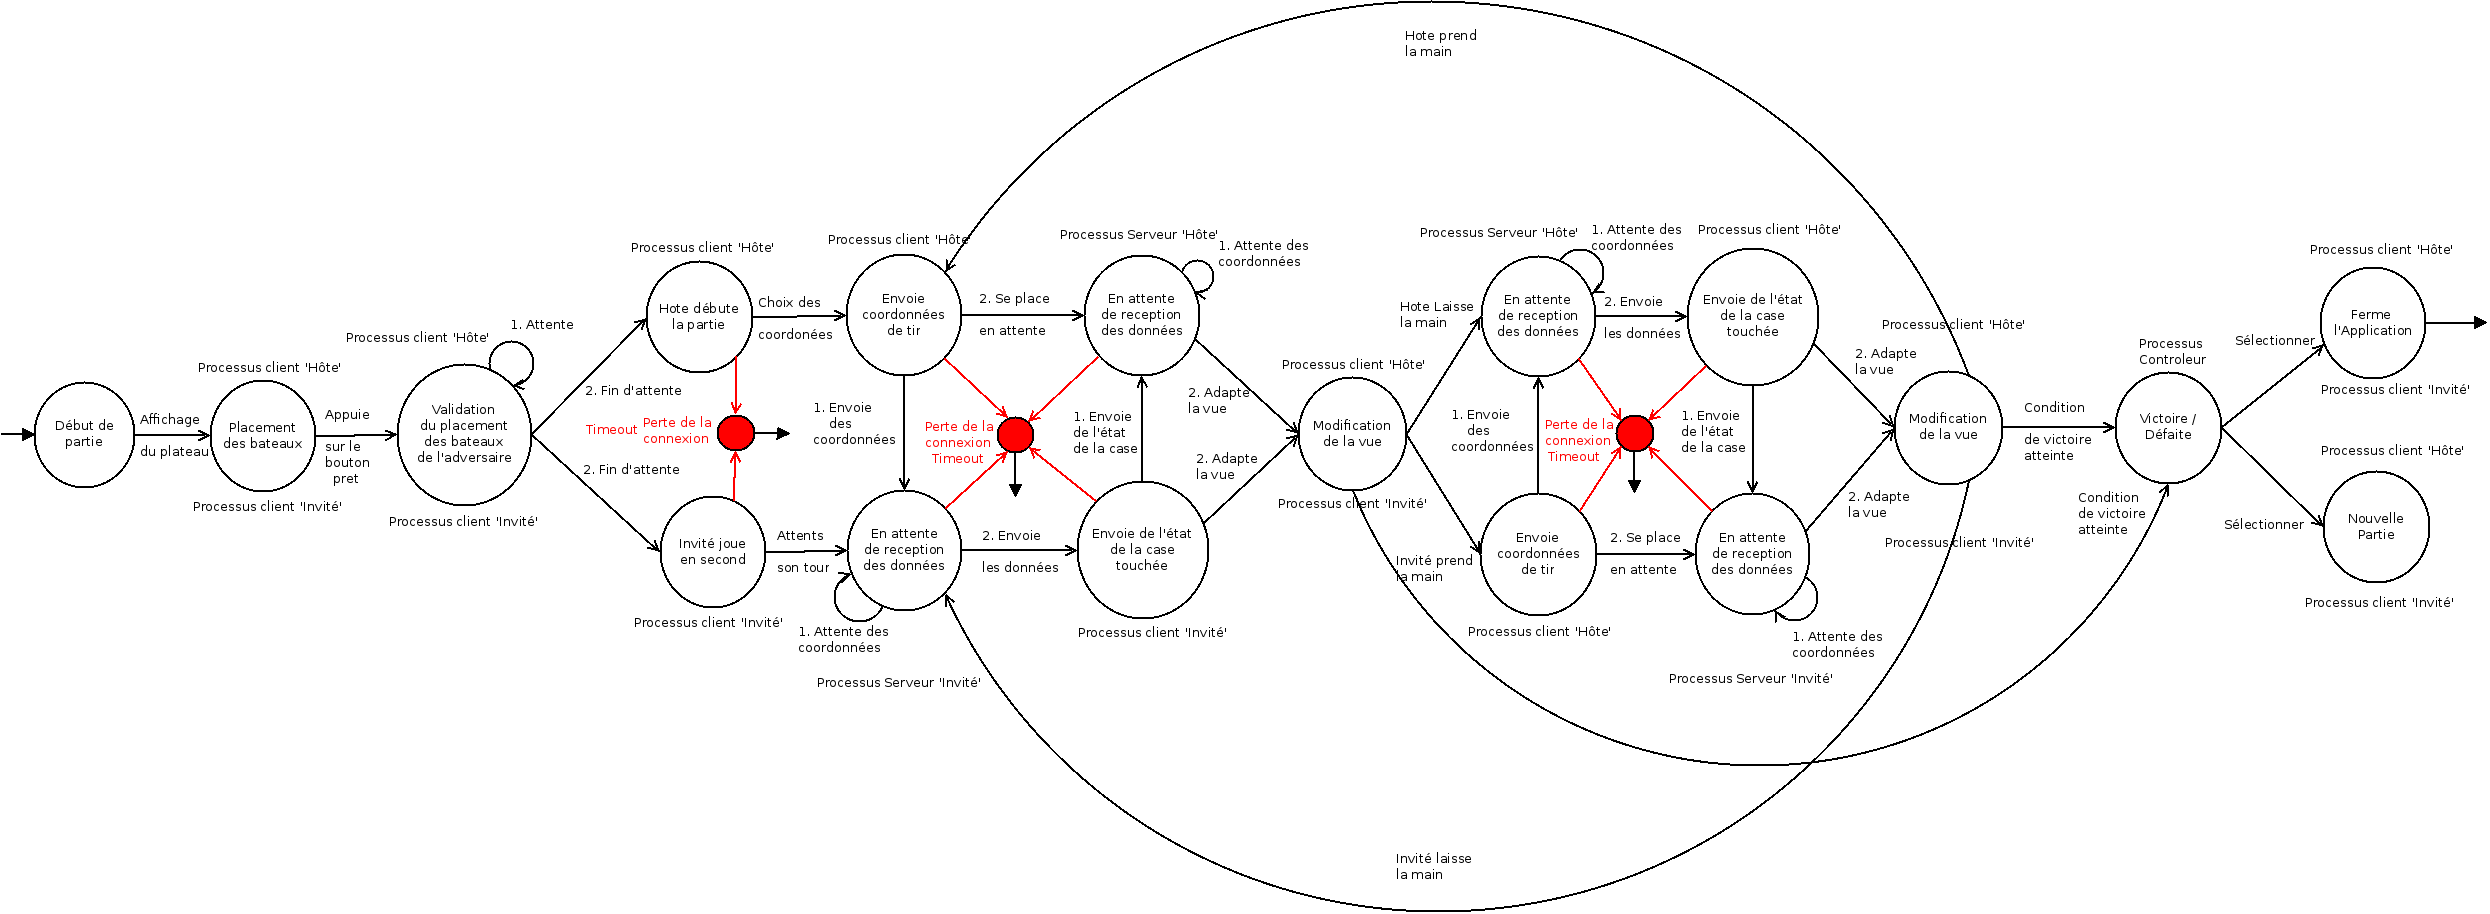
\includegraphics [width=215mm]{images/data_exhange_between_players.png}
    \caption{Schéma représentant le protocole d'échange de données entre deux joueurs}
    \label{connection}
\end{sidewaysfigure}

\end{appendices}

\end{document}

